\chapter{Requirements Analysis}
\label{ch:Requirements_Analysis}

This chapter will discuss the high-level decisions made to narrow the scope of the project. 

Even though Section \ref{sec:Objectives} very clearly specified the objectives that this project aimed for, it gave us free rein on what methods and techniques we utilised to achieve them. 

These decisions, largely influenced by the background research found in Chapter \ref{ch:Background}, could be roughly split up into two distinct but interconnected sections that would determine the project's direction.

It should also be noted that some of these decisions, made early on in the project's life-cycle, were later revisited and updated accordingly, given our improved understanding of the problem and the methods we had used up to that point.

\section{Model Decisions}

The decisions that needed to be made for this section were the following:

\begin{itemize}
    \item
    Which machine learning library would we use.
    \item
    What type of models would we build.
    \item
    What metrics and methods would we use to evaluate the models' predictive performance.
    \item
    How would these models be optimised.
    \item
    How would we test these models for robustness.
    \item
    How would we make the models' predictions more interpretable.
    \item
    How would we present our findings.
\end{itemize}

\subsection{Machine Learning Library}

We decided to use scikit-learn \citep{scikit-learn} to build our models, as it is one of the best machine learning libraries with excellent documentation and tutorials available. 

\subsection{Model Types}
\label{subsec:Model_Types}

We had initially chosen to only build classification models but after going through the publicly available data sets, provided by the studies and papers we already discussed in Chapter \ref{ch:Background}, and noticing that the logBB values of some drugs and compounds were also provided in addition to their ability to penetrate the blood-brain barrier or not, we chose to build both classification and regression models.

We decided to use multiple metrics for both types of models to evaluate their performance. This was done as it is generally viewed as good practice and gives a more complete view of the models' performance and limitations. 

\subsection{Classification Metrics}

The classification models would be evaluated based on Precision, Recall, F1 Score, Accuracy and Matthews correlation coefficient (MCC). These metrics make use of the confusion matrix, which is a table, as shown in Figure \ref{fig:Confusion_Matrix}, that records the total number of true positives (TP) and negatives (TN) and false positives (FP) and negatives (FN).

Precision measures how many of the positive predictions made by the classifier were actually positive \citep{Precision}. It ranges from 0 to +1, with +1 being the best and 0 being the worst.

$$Precision =  \frac{TP}{TP + FP}$$

Recall, also known as Sensitivity, measures how many of the actual positives were labelled as positive by our classifier \citep{Recall}. It ranges from 0 to +1, with +1 being the best and 0 being the worst.
$$Recall = \frac{TP}{TP + FN}$$

F1 score is the harmonic mean of precision and recall \citep{F1}. Other variations exist where precision or recall can be given more or less weight. It ranges from 0 to +1, with +1 being the best and 0 being the worst.
$$F1 = \frac{2 * (precision * recall)}{precision + recall}$$
\label{itm:F1}

Accuracy measures the number of correct predictions made by the classifier \citep{Accuracy}. It ranges from 0 to +1, with +1 being the best and 0 being the worst.
$$Accuracy = \frac{TP + TN}{TP + TN + FP + FN} $$

Matthews correlation coefficient (MCC), also known as Phi coefficient, essentially calculates the correlation between the predicted and true values \citep{MCC}. It takes into account the whole confusion matrix and is generally thought of as a particularly useful metric, even when the classes are imbalanced.

MCC has a range of -1 to +1. A coefficient of +1 indicates a perfect relation between predicted and true values, 0 that our model is randomly guessing, and -1 an inverse relationship between predicted and true values \citep{MCC2}.

$$MCC = \frac{TP*TN - FP*FN}{\sqrt{(TP+FP)(TP+FN)(TN+FP)(TN+FN)}}$$

\newpage

\begin{figure}[!htb]
    \centering
    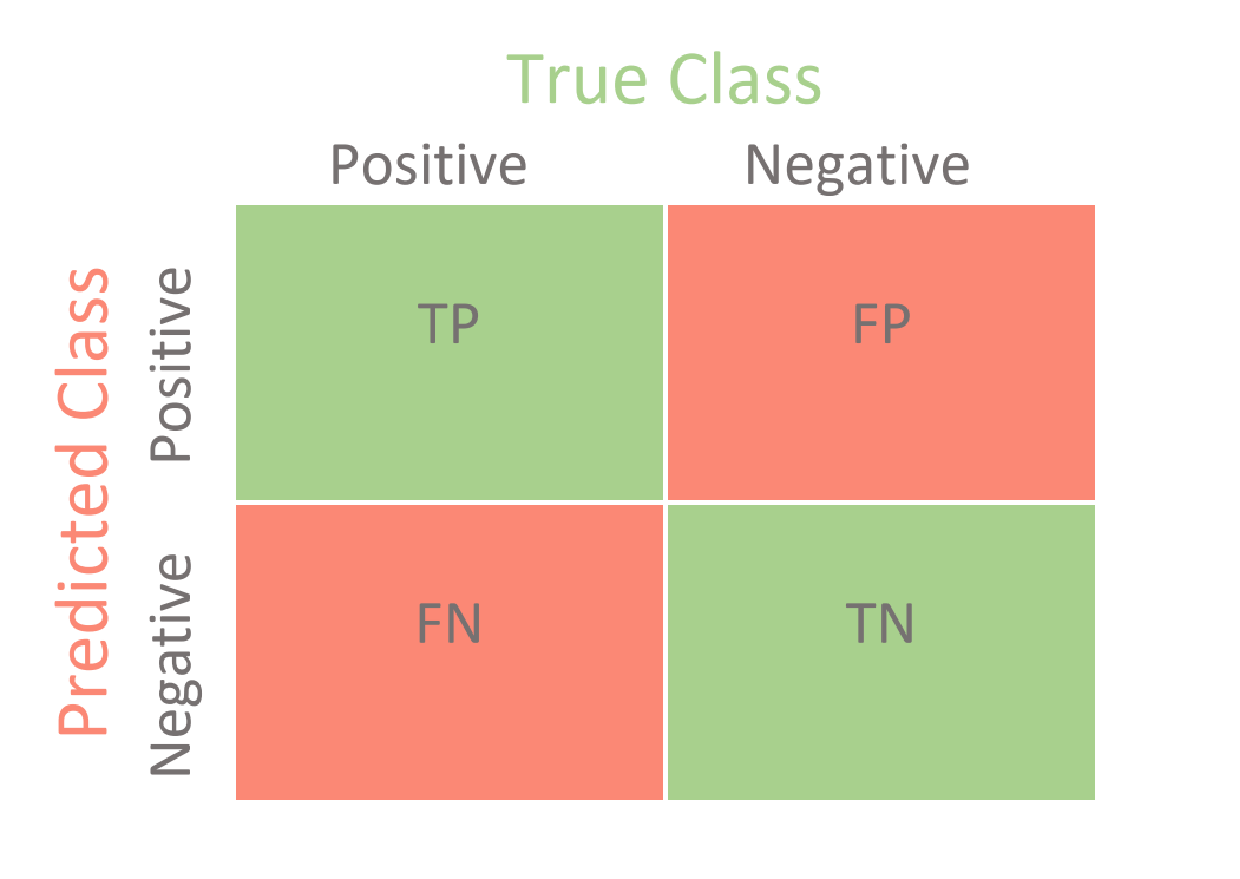
\includegraphics[width=0.8\linewidth]{images/TDS_Confusion_Matrix.pdf}    

    \caption{Figure taken from \citet{Confusion_Matrix} showcasing the confusion matrix for a binary classification problem.}

    \label{fig:Confusion_Matrix} 
\end{figure}

\subsection{Regression Metrics}

The regression models would be evaluated based on Negated Mean Absolute Error and R2 Score.

\newenvironment{conditions}
  {\par\vspace{\abovedisplayskip}\noindent\begin{tabular}{>{$}l<{$} @{${}={}$} l}}
  {\end{tabular}\par\vspace{\belowdisplayskip}}
  
The Mean Absolute Error (MAE) calculates exactly what its name suggests. It finds the absolute error, also known as the difference, between the predicted and the true value for all data points in a set, sums them up and then calculates their mean \citep{MAE}. It has a range of 0 to +$\infty$, with 0 being the best score.

The Negated Mean Absolute Error just adds a negative sign in front of MAE. It has a range of -$\infty$ to 0, with 0 again being the best score. We chose to use this variation so that all the metrics followed the same 'greater is better' principle, thus making their interpretation easier.

$$\text{Mean Absolute Error} (y,\hat{y}) = (\frac{1}{n})\sum_{i=1}^{n}\left | y_{i} - \hat{y}_{i} \right | $$

where: 
\begin{conditions}
n & number of samples\\
y & true values \\
\hat{y} & predicted values
\end{conditions}

The R2 score measures how good the regression line fits our data \citep{R2}. It compares the fit to a baseline model that essentially always predicts the mean of the true values \citep{R2_2}. Generally, it ranges from 0 to +1, with +1 being the best score, but it can also become negative, indicating a worse model.

$$\text{R2 Score} (y,\hat{y}) = 1 - (\frac{\sum_{i=1}^{n}(y_{i} - \hat{y}_{i})^2}{\sum_{i=1}^{n}(y_{i} - \bar{y})^2})$$

where: 
\begin{conditions}
n & number of samples\\
y & true values \\
\hat{y} & predicted values \\
\bar{y} & mean of true values
\end{conditions}

\subsection{Model Evaluation Methods}

We decided to use holdout test sets and dummy models to evaluate our models.

Holdout test sets are untouched subsets of the data, meaning they have not been used for training or validation purposes,  that are specifically employed to estimate the model's performance on unseen real-world data.

Dummy models usually predict the most frequent class in our data, in the case of classification models, and the mean of our labels, what we are trying to predict, in the case of regression models, although there are multiple variations \citep{DummyClassifier, DummyRegressor}. These would serve as the baselines for our models.

\subsection{Model Optimisation}
\label{subsec:Model_Optimisation}

The models' hyper-parameters would be tuned using scikit-learn's GridSearch function \citep{GridSearch} which makes use of cross-validation to optimise the models for a specific metric. 

GridSearch essentially splits the data provided into multiple training and validation subsets, with the default being five unless otherwise specified. Then it iteratively goes through the pairs of training and validation subsets, training the model on the training subset using a combination of its hyper-parameters and then uses the trained model to make predictions on the validation set and calculates a score. Once all the pairs have been used, it calculates the mean validation score, moves on to the following combination of hyper-parameters, and repeats the process until all the combinations have been exhausted.

The function can then return the scores for all combinations of hyper-parameters for inspection and the model with the best mean validation score, along with the hyper-parameters used to train it.

The metrics we chose to optimise our models were the F1 score for the classification models and the R2 score for the regression ones.

\subsection{Model Robustness}
\label{subsec:Robustness}

To check the robustness of the models, we would use scikit-learn's Permutation Test Score function. \citep{Permutation_Test_Score}. This process is also known as y-scrambling.

This is essentially a statistical hypothesis test with a null hypothesis stating that a statistical relationship does not exist between the features and label using our model and an alternative hypothesis stating that a statistical relationship does indeed exist using our model.

Again this function just as GridSearch, found in Subsection \ref{subsec:Model_Optimisation}, uses cross-validation. It iteratively goes through the pairs of training and validation sets and, for each permutation, randomly reorders the labels. Unless otherwise specified, this is repeated 100 times, removing any relationship between the features and the labels.

It returns a p-value which represents the probability that the model's predictions are just the result of random chance. The p-value is just the fraction of permutations that their mean validation score is better than the mean validation score obtained using the original data that correctly matches the features with their labels \citep{Permutation_Test_Score_Explanation}. Generally, if this p-value is less than or equal to 0.05, we assume that we have a statistically significant result and reject the null hypothesis.

\subsection{Model Interpretability}
\label{subsec:Interpretability}

Model interpretability was one of the last and most challenging questions we tackled. So we decided to try and make our models more interpretable to shine some light in their inner workings and instil some confidence in their predictions, or at the very least help whoever is using them understand what led to that prediction.

We decided to use \citet{ELI5} to examine the weights of the models' features and \citet{LIME} to explain how those features and their values led to a specific prediction.

\subsection{Presenting Findings}

The presentation of our findings was in flux until the very last stages of the project. We had previously discussed that, at the very least, we should produce a notebook or a simplistic web app. In the end, we decided to create a very simple \citet{Streamlit} web application that showcases the project's processes and the models produced.

\section{Data Set Decisions}
\label{sec:Dataset_Decisions}

The decisions that needed to be made for this category were the following:

\begin{itemize}
    \item
    What would we use as our label.
    \item
    What chemical descriptors would we use.
    \item
    Could we make use of other drug characteristics.
    \item
    How would the data set be built, and more specifically, what sources and methods would we use to create it.
\end{itemize}

\subsection{Labels}
\label{subsec:Labels}

For our classification models, the label would be whether a drug or compound can penetrate the blood-brain barrier or not, designated by a 1 and a 0, respectively, and for our regression models, the label would be the logBB value.

\subsection{Chemical Descriptors}
\label{subsec:Chemical_Descriptors}

After concluding our background research, discussed in Chapter \ref{ch:Background}, we had decided to use a tiny number of widely available chemical descriptors, specifically the same ones used by \citet{Saber2020}. 

Naturally, one of the world's largest and freely accessible databases of chemical information, \citet{PubChem}, was an excellent fit for our needs. However, we early on noticed that pKa (strongest base) and pKa (strongest acid) were not available, two of the eight chemical descriptors we wanted to use, and instead, we just had access to the pKa. So we made the decision to make use of this pKa descriptor, but we then observed that for the vast majority of drugs and compounds, this chemical descriptor was unavailable, so we finally settled on outright removing it from the data set altogether, reducing the number of chemical descriptors from 8 to 6.

The chemical descriptors we ended up using were:

\begin{itemize}
    \item
    Molecular weight (MW)
    \item
    Topological polar surface area (TPSA)
    \item
    Octanol-water partition coefficient (XLogP)
    \item
    Number of hydrogen-bond donors (NHD)
    \item
    Number of hydrogen-bond acceptors (NHA)
    \item
   Number of rotatable bonds (NRB)
\end{itemize}

\subsection{Other Characteristics}
\label{subsec:Other_Characteristics}

Inspired by the novel approach used by \citet{Gao2017} to solve the problem, as discussed in Section \ref{sec:Novel_Approach}, we also decided to make use of the recorded side effects and indications of drugs and compounds stored in the \citet{SIDER} database, to test whether the addition to the chemical descriptors improved the predictive performance of our models or not.

Side effects and indications pointing to central nervous system (CNS) issues should act as powerful indicators that a drug or compound can successfully penetrate the blood-brain barrier. However, just as it was already mentioned in Section \ref{sec:Important_Chemical_Descriptors} BBB+ drugs and compounds can have no effect on the CNS, making it harder to detect blood-brain barrier penetration solely through the usage of side effects and indications as features. 

\subsection{Data Set Sources}

To create our data set, we decided to combine the publicly available data sets already provided by the studies and papers we previously discussed in Chapter \ref{ch:Background} and augment them to suit our own needs. 

As mentioned in Subsections \ref{subsec:Chemical_Descriptors} and \ref{subsec:Other_Characteristics} we would make use of the \citet{PubChem} database to retrieve the chemical descriptors for each drug and compound and the \citet{SIDER} database to retrieve the side effects and indications.

We also aimed to further expand the size of the data set using straightforward text mining techniques on google searches about blood-brain permeability. Unfortunately, this was proven to be noisy and unreliable. However, the techniques and methods developed were easily repurposed on searches performed on medical APIs, like \citet{PubMedAPI} and \citet{SpringerAPI}, which proved to be much more reliable.


